\icode{E-MI-SI-L2-261031-002}
如图所示是粉刷墙壁的涂料滚的示意图，撑竿的重量和墙壁的摩擦均不计，而且撑竿足够长，粉刷工人站在离墙壁某一距离处缓缓上推涂料滚，使撑竿与墙壁间的夹角越来越小。该过程中撑竿对涂料滚的推力为\(F\)，墙壁对涂料滚的支持力为\(F_N\)，下列说法正确的是\paren[]

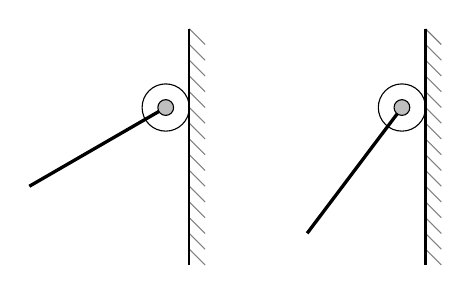
\begin{tikzpicture}[font=\scriptsize]
	\begin{scope}
		\draw[very thick] (0,0)--(-150:2);
		\draw[fill=gray!50] (0,0) circle(.1);
		\draw (0,0) circle(.3);
		\foreach \y in {1,.8,...,-1.8}
			\draw[gray] (.3,\y)--++(.2,-.2);
		\draw[thick] (.3,1)--(.3,-2);
	\end{scope}
	\begin{scope}[xshift=3cm]
		\draw[very thick] (0,0)--(-127:2);
		\draw[fill=gray!50] (0,0) circle(.1);
		\draw (0,0) circle(.3);
		\foreach \y in {1,.8,...,-1.8}
			\draw[gray] (.3,\y)--++(.2,-.2);
		\draw[thick] (.3,1)--(.3,-2);
	\end{scope}
\end{tikzpicture}
\begin{choices}
	\item\(F\)、\(F_N\)均减小
	\item\(F\)、\(F_N\)均增大
	\item\(F\)减小，\(F_N\)增大
	\item\(F\)增大，\(F_N\)减小
\end{choices}
\begin{answer}
	A\qquad 提示：受力分析，并构建力的矢量三角形
\end{answer}